\documentclass[journal,12pt,twocolumn]{IEEEtran}
%
\usepackage{setspace}
\usepackage{gensymb}
%\doublespacing
\singlespacing

%\usepackage{graphicx}
%\usepackage{amssymb}
%\usepackage{relsize}
\usepackage[cmex10]{amsmath}
%\usepackage{amsthm}
%\interdisplaylinepenalty=2500
%\savesymbol{iint}
%\usepackage{txfonts}
%\restoresymbol{TXF}{iint}
%\usepackage{wasysym}
\usepackage{amsthm}
%\usepackage{iithtlc}
\usepackage{mathrsfs}
\usepackage{txfonts}
\usepackage{stfloats}
\usepackage{steinmetz}
\usepackage{bm}
\usepackage{cite}
\usepackage{cases}
\usepackage{subfig}
%\usepackage{xtab}
\usepackage{longtable}
\usepackage{multirow}
%\usepackage{algorithm}
%\usepackage{algpseudocode}
\usepackage{enumitem}
\usepackage{mathtools}
\usepackage{tikz}
\usepackage{circuitikz}
\usepackage{verbatim}
\usepackage{tfrupee}
\usepackage[breaklinks=true]{hyperref}
%\usepackage{stmaryrd}
\usepackage{tkz-euclide} % loads  TikZ and tkz-base
%\usetkzobj{all}
\usepackage{listings}
    \usepackage{color}                                            %%
    \usepackage{array}                                            %%
    \usepackage{longtable}                                        %%
    \usepackage{calc}                                             %%
    \usepackage{multirow}                                         %%
    \usepackage{hhline}                                           %%
    \usepackage{ifthen}                                           %%
  %optionally (for landscape tables embedded in another document): %%
    \usepackage{lscape}     
\usepackage{multicol}
\usepackage{chngcntr}
%\usepackage{enumerate}

%\usepackage{wasysym}
%\newcounter{MYtempeqncnt}
\DeclareMathOperator*{\Res}{Res}
%\renewcommand{\baselinestretch}{2}
\renewcommand\thesection{\arabic{section}}
\renewcommand\thesubsection{\thesection.\arabic{subsection}}
\renewcommand\thesubsubsection{\thesubsection.\arabic{subsubsection}}

\renewcommand\thesectiondis{\arabic{section}}
\renewcommand\thesubsectiondis{\thesectiondis.\arabic{subsection}}
\renewcommand\thesubsubsectiondis{\thesubsectiondis.\arabic{subsubsection}}

% correct bad hyphenation here
\hyphenation{op-tical net-works semi-conduc-tor}
\def\inputGnumericTable{}                                 %%

\lstset{
%language=C,
frame=single, 
breaklines=true,
columns=fullflexible
}
%\lstset{
%language=tex,
%frame=single, 
%breaklines=true
%}

\begin{document}
%


\newtheorem{theorem}{Theorem}[section]
\newtheorem{problem}{Problem}
\newtheorem{proposition}{Proposition}[section]
\newtheorem{lemma}{Lemma}[section]
\newtheorem{corollary}[theorem]{Corollary}
\newtheorem{example}{Example}[section]
\newtheorem{definition}[problem]{Definition}
%\newtheorem{thm}{Theorem}[section] 
%\newtheorem{defn}[thm]{Definition}
%\newtheorem{algorithm}{Algorithm}[section]
%\newtheorem{cor}{Corollary}
\newcommand{\BEQA}{\begin{eqnarray}}
\newcommand{\EEQA}{\end{eqnarray}}
\newcommand{\define}{\stackrel{\triangle}{=}}

\bibliographystyle{IEEEtran}
%\bibliographystyle{ieeetr}


\providecommand{\mbf}{\mathbf}
\providecommand{\pr}[1]{\ensuremath{\Pr\left(#1\right)}}
\providecommand{\qfunc}[1]{\ensuremath{Q\left(#1\right)}}
\providecommand{\sbrak}[1]{\ensuremath{{}\left[#1\right]}}
\providecommand{\lsbrak}[1]{\ensuremath{{}\left[#1\right.}}
\providecommand{\rsbrak}[1]{\ensuremath{{}\left.#1\right]}}
\providecommand{\brak}[1]{\ensuremath{\left(#1\right)}}
\providecommand{\lbrak}[1]{\ensuremath{\left(#1\right.}}
\providecommand{\rbrak}[1]{\ensuremath{\left.#1\right)}}
\providecommand{\cbrak}[1]{\ensuremath{\left\{#1\right\}}}
\providecommand{\lcbrak}[1]{\ensuremath{\left\{#1\right.}}
\providecommand{\rcbrak}[1]{\ensuremath{\left.#1\right\}}}
\theoremstyle{remark}
\newtheorem{rem}{Remark}
\newcommand{\sgn}{\mathop{\mathrm{sgn}}}
\providecommand{\abs}[1]{\left\vert#1\right\vert}
\providecommand{\res}[1]{\Res\displaylimits_{#1}} 
\providecommand{\norm}[1]{\left\lVert#1\right\rVert}
%\providecommand{\norm}[1]{\lVert#1\rVert}
\providecommand{\mtx}[1]{\mathbf{#1}}
\providecommand{\mean}[1]{E\left[ #1 \right]}
\providecommand{\fourier}{\overset{\mathcal{F}}{ \rightleftharpoons}}
%\providecommand{\hilbert}{\overset{\mathcal{H}}{ \rightleftharpoons}}
\providecommand{\system}{\overset{\mathcal{H}}{ \longleftrightarrow}}
	%\newcommand{\solution}[2]{\textbf{Solution:}{#1}}
\newcommand{\solution}{\noindent \textbf{Solution: }}
\newcommand{\cosec}{\,\text{cosec}\,}
\providecommand{\dec}[2]{\ensuremath{\overset{#1}{\underset{#2}{\gtrless}}}}
\newcommand{\myvec}[1]{\ensuremath{\begin{pmatrix}#1\end{pmatrix}}}
\newcommand{\mydet}[1]{\ensuremath{\begin{vmatrix}#1\end{vmatrix}}}
%\numberwithin{equation}{section}
\numberwithin{equation}{subsection}
%\numberwithin{problem}{section}
%\numberwithin{definition}{section}
\makeatletter
\@addtoreset{figure}{problem}
\makeatother

\let\StandardTheFigure\thefigure
\let\vec\mathbf
%\renewcommand{\thefigure}{\theproblem.\arabic{figure}}
\renewcommand{\thefigure}{\theproblem}
%\setlist[enumerate,1]{before=\renewcommand\theequation{\theenumi.\arabic{equation}}
%\counterwithin{equation}{enumi}


%\renewcommand{\theequation}{\arabic{subsection}.\arabic{equation}}

\def\putbox#1#2#3{\makebox[0in][l]{\makebox[#1][l]{}\raisebox{\baselineskip}[0in][0in]{\raisebox{#2}[0in][0in]{#3}}}}
     \def\rightbox#1{\makebox[0in][r]{#1}}
     \def\centbox#1{\makebox[0in]{#1}}
     \def\topbox#1{\raisebox{-\baselineskip}[0in][0in]{#1}}
     \def\midbox#1{\raisebox{-0.5\baselineskip}[0in][0in]{#1}}

\vspace{3cm}

\title{
	%\logo{
%Computational Approach to School Geometry
Points and Vectors
%	}
}
\author{ G V V Sharma$^{*}$% <-this % stops a space
	\thanks{*The author is with the Department
		of Electrical Engineering, Indian Institute of Technology, Hyderabad
		502285 India e-mail:  gadepall@iith.ac.in. All content in this manual is released under GNU GPL.  Free and open source.}
	
}	
%\title{
%	\logo{Matrix Analysis through Octave}{\begin{center}\includegraphics[scale=.24]{tlc}\end{center}}{}{HAMDSP}
%}


% paper title
% can use linebreaks \\ within to get better formatting as desired
%\title{Matrix Analysis through Octave}
%
%
% author names and IEEE memberships
% note positions of commas and nonbreaking spaces ( ~ ) LaTeX will not break
% a structure at a ~ so this keeps an author's name from being broken across
% two lines.
% use \thanks{} to gain access to the first footnote area
% a separate \thanks must be used for each paragraph as LaTeX2e's \thanks
% was not built to handle multiple paragraphs
%

%\author{<-this % stops a space
%\thanks{}}
%}
% note the % following the last \IEEEmembership and also \thanks - 
% these prevent an unwanted space from occurring between the last author name
% and the end of the author line. i.e., if you had this:
% 
% \author{....lastname \thanks{...} \thanks{...} }
%                     ^------------^------------^----Do not want these spaces!
%
% a space would be appended to the last name and could cause every name on that
% line to be shifted left slightly. This is one of those "LaTeX things". For
% instance, "\textbf{A} \textbf{B}" will typeset as "A B" not "AB". To get
% "AB" then you have to do: "\textbf{A}\textbf{B}"
% \thanks is no different in this regard, so shield the last } of each \thanks
% that ends a line with a % and do not let a space in before the next \thanks.
% Spaces after \IEEEmembership other than the last one are OK (and needed) as
% you are supposed to have spaces between the names. For what it is worth,
% this is a minor point as most people would not even notice if the said evil
% space somehow managed to creep in.



% The paper headers
%\markboth{Journal of \LaTeX\ Class Files,~Vol.~6, No.~1, January~2007}%
%{Shell \MakeLowercase{\textit{et al.}}: Bare Demo of IEEEtran.cls for Journals}
% The only time the second header will appear is for the odd numbered pages
% after the title page when using the twoside option.
% 
% *** Note that you probably will NOT want to include the author's ***
% *** name in the headers of peer review papers.                   ***
% You can use \ifCLASSOPTIONpeerreview for conditional compilation here if
% you desire.




% If you want to put a publisher's ID mark on the page you can do it like
% this:
%\IEEEpubid{0000--0000/00\$00.00~\copyright~2007 IEEE}
% Remember, if you use this you must call \IEEEpubidadjcol in the second
% column for its text to clear the IEEEpubid mark.



% make the title area
\maketitle

\newpage

\tableofcontents

\bigskip

\renewcommand{\thefigure}{\theenumi}
\renewcommand{\thetable}{\theenumi}
%\renewcommand{\theequation}{\theenumi}

%\begin{abstract}
%%\boldmath
%In this letter, an algorithm for evaluating the exact analytical bit error rate  (BER)  for the piecewise linear (PL) combiner for  multiple relays is presented. Previous results were available only for upto three relays. The algorithm is unique in the sense that  the actual mathematical expressions, that are prohibitively large, need not be explicitly obtained. The diversity gain due to multiple relays is shown through plots of the analytical BER, well supported by simulations. 
%
%\end{abstract}
% IEEEtran.cls defaults to using nonbold math in the Abstract.
% This preserves the distinction between vectors and scalars. However,
% if the journal you are submitting to favors bold math in the abstract,
% then you can use LaTeX's standard command \boldmath at the very start
% of the abstract to achieve this. Many IEEE journals frown on math
% in the abstract anyway.

% Note that keywords are not normally used for peerreview papers.
%\begin{IEEEkeywords}
%Cooperative diversity, decode and forward, piecewise linear
%\end{IEEEkeywords}



% For peer review papers, you can put extra information on the cover
% page as needed:
% \ifCLASSOPTIONpeerreview
% \begin{center} \bfseries EDICS Category: 3-BBND \end{center}
% \fi
%
% For peerreview papers, this IEEEtran command inserts a page break and
% creates the second title. It will be ignored for other modes.
%\IEEEpeerreviewmaketitle

\begin{abstract}
This book provides a computational approach to school geometry based on the NCERT textbooks from Class 6-12.  Links to sample Python codes are available in the text.  
\end{abstract}
Download python codes using 
\begin{lstlisting}
svn co https://github.com/gadepall/school/trunk/ncert/computation/codes
\end{lstlisting}

%\section{Triangle}
\section{Examples}
\renewcommand{\theequation}{\theenumi}
\begin{enumerate}[label=\thesection.\arabic*.,ref=\thesection.\theenumi]
\numberwithin{equation}{enumi}

%\renewcommand{\theequation}{\theenumi}
%\begin{enumerate}[label=\thesubsection.\arabic*.,ref=\thesubsection.\theenumi]
%\numberwithin{equation}{enumi}
%
\item Show that the points 
\begin{align}
\vec{A} = \myvec{2\\-1 \\1},
\vec{B} = \myvec{1\\-3 \\-5},
\vec{C} = \myvec{3\\ -4\\-4}
\end{align}
%
are the vertices of a right angled triangle.
\\
\solution 
The following code plots Fig. \ref{fig:triangle_3d}
%
\begin{lstlisting}
codes/triangle/triangle_3d.py
\end{lstlisting}
%
\begin{figure}[!ht]
\includegraphics[width=\columnwidth]{./triangle/figs/triangle_3d.eps}
\caption{}
\label{fig:triangle_3d}
\end{figure}
%
From the figure, it appears that $\triangle ABC$ is right angled at $\vec{C}$.  Since 
\begin{align}
\brak{\vec{A}-\vec{C}}^T\brak{\vec{B}-\vec{C}}&=0
\end{align}
%
it is proved that the triangle is indeed right angled.
\item Do the points $\vec{A}=\myvec{3\\2}, \vec{B}=\myvec{-2\\-3}, \vec{C}=\myvec{2\\3} $ form a triangle?  If so, name the type of triangle formed.
\label{prob:tri_exam_coll_pts}
%
\\
\solution 

The direction vectors of $AB$ and $BC$ are 
\begin{align}
\label{eq:tri_geo_ex_baorth}
\vec{B}-\vec{A} &= \myvec{-5\\-5}
\\
\vec{C}-\vec{A} &= \myvec{-1\\1}
\label{eq:tri_geo_ex_caorth}
\end{align}
%
If $\vec{A}, \vec{B}, \vec{C}$ form a line, then, $AB$ and $AC$ should have the same direction vector. Hence, there exists a $k$ such that
\begin{align}
\vec{B}-\vec{A} &= k\brak{\vec{C}-\vec{B}}
\\
\implies \vec{B} &= \frac{k\vec{C} +\vec{A}}{k+1}
\label{eq:tri_geo_ex_caorth_section}
\end{align}
%
Since 
\begin{align}
\vec{B}-\vec{A} \ne k\brak{\vec{C}-\vec{A}},
\end{align}
%
the points are not collinear and form a triangle.  An alternative method is to create the matrix
\begin{align}
\label{eq:tri_geo_ex_diff_mat}
\vec{M} = \myvec{\vec{B}-\vec{A} & \vec{B}-\vec{A}}^T 
\end{align}
%
If $rank(\vec{M}) = 1$, the points are collinear.  The rank of a matrix is the number of nonzero rows left after doing row operations.  In this problem, 
%
\begin{align}
\vec{M} = \myvec{-5 & -5\\-1 & 1}\xleftrightarrow {R_2\leftarrow 5R_2-R_1}\myvec{-5 & -5\\0 & 10}
\\
\implies rank(\vec{M}) = 2
\end{align}
%
as the number of non zero rows is 2.
The following code plots Fig. \ref{fig:check_tri}
%
\begin{lstlisting}
codes/triangle/check_tri.py
\end{lstlisting}
%
\begin{figure}[!ht]
\includegraphics[width=\columnwidth]{./triangle/figs/check_tri.eps}
\caption{}
\label{fig:check_tri}
\end{figure}
%
From the figure, it appears that $\triangle ABC$ is right angled, with $BC$ as the hypotenuse.  From Baudhayana's theorem, this would be true if 
\begin{align}
\norm{\vec{B}-\vec{A}}^2+\norm{\vec{C}-\vec{A}}^2&=\norm{\vec{B}-\vec{C}}^2
\end{align}
which can be expressed as
\begin{multline}
\norm{\vec{A}}^2 + \norm{\vec{C}}^2 - 2\vec{A}^T\vec{C}+
\norm{\vec{A}}^2 + \norm{\vec{B}}^2 - 2\vec{A}^T\vec{B}
\\
=
\norm{\vec{B}}^2 + \norm{\vec{C}}^2 - 2\vec{B}^T\vec{C}
\end{multline}
%
to obtain 
\begin{align}
\label{eq:tri_geo_ex_orth}
\brak{\vec{B}-\vec{A}}^T\brak{\vec{C}-\vec{A}}&=0
\end{align}
%
after simplification.  From \eqref{eq:tri_geo_ex_baorth} and \eqref{eq:tri_geo_ex_caorth}, it is easy to verify that 
\begin{align}
\label{eq:tri_geo_ex_orth_sol}
\brak{\vec{B}-\vec{A}}^T\brak{\vec{C}-\vec{A}}=
 \myvec{-5 & -5}\myvec{-1\\1} = 0
\end{align}
satisfying
\eqref{eq:tri_geo_ex_orth}. Thus,  $\triangle ABC$ is right angled at $\vec{A}$.
%
%
%\item Area of a triangle is half the product of its base and the corresponding altitude. 
%%
%\\
%\solution First, we consider the right angled triangle in Fig\ref{fig:tri_right_area}. By definition, the area of the rectangle $ABCD$ is $ac$.  Also, The rectangle is a sum of two congruent triangles $ABC$ and $ADC$.  Thus,
%%
%\begin{align}
%\text{ar}\triangle ABC=\text{ar}\triangle ADC = \frac{1}{2}ac
%\end{align} 
%%
%\begin{figure}[!ht]
%\includegraphics[width=\columnwidth]{./triangle/figs/tri_right_area.eps}
%\caption{}
%\label{fig:tri_right_area}
%\end{figure}
%%
%For any $\triangle ABC$, as shown in Fig.  \ref{fig:tri_area}, the area can be obtained as
%%
%\begin{align}
%\text{ar}\triangle ABC&=\frac{1}{2}xh+\frac{1}{2}yh 
%\\
%\frac{1}{2}\brak{x+y}h = \frac{1}{2}ah
%\end{align} 
%%

%
%\begin{figure}[!ht]
%\includegraphics[width=\columnwidth]{./triangle/figs/tri_area.eps}
%\caption{}
%\label{fig:tri_area}
%\end{figure}
%
\item Find the area of a triangle whose vertices are 
$\vec{A}=\myvec{1\\-1}, 
\vec{B} = \myvec{-4\\6}$ and
$ 
\vec{C} = \myvec{-3\\-5}
$.
%
\\
\solution
  Using Hero's formula, the following code computes the area of the  triangle as 24.
%
\begin{lstlisting}
codes/triangle/area_tri.py
\end{lstlisting}
%
%\item A median of a triangle divides it into two triangles of equal areas.
%\\
%\solution In $\triangle ABC$, let $AD$
%
\item Find the area of a triangle formed by the vertices $\vec{A}=\myvec{5\\2}, \vec{B}=\myvec{4\\7}, \vec{C}=\myvec{7\\-4}$.
%\\
\solution  The area of $\triangle ABC$ is also obtained  in terms of the  {\em magnitude} of the determinant of the matrix $\vec{M}$ in  \eqref{eq:tri_geo_ex_diff_mat} as
%
\begin{align}
\frac{1}{2}\mydet{\vec{M}}
\end{align}
The computation is done in \textbf{area\_tri.py}
\item Find the area of a triangle formed by the points $\vec{P}=\myvec{-1.5\\3}, \vec{Q}=\myvec{6\\-2}, \vec{R}=\myvec{-3\\4}$.
\\
\solution Another formula for the area of $\triangle ABC$  is
%
\begin{align}
\frac{1}{2}\mydet{1 & 1 & 1\\ \vec{A} & \vec{B} & \vec{C} }
\end{align}
%
\item Find the area of a triangle having the points
%
\begin{align}
\vec{A} = \myvec{1\\1 \\1},
\vec{B} = \myvec{1\\2 \\3},
\vec{C} = \myvec{2\\ 3\\1}
\end{align}
%
as its vertices.
\\
\solution The area of a triangle using the {\em vector product} is obtained as
\begin{align}
\frac{1}{2}\norm{\brak{\vec{B}-\vec{A}}\times \brak{\vec{C}-\vec{A}}}
\end{align}
%
For any two vectors $\vec{a}=\myvec{a_1\\a_2\\a_3}, \vec{b}=\myvec{b_1\\b_2\\b_3}$, 
\begin{align}
\label{eq:tri_cross_prod}
\vec{a}\times \vec{b} = \myvec{0 & -a_3 & a_2 \\ a_3 & 0 & -a_1 \\ -a_2 & a_1 & 0}\myvec{b_1\\b_2\\b_3}
\end{align}
%
The following code computes the area using the vector product.
%
\begin{lstlisting}
codes/triangle/area_tri_vec.py
\end{lstlisting}
%
%
\item The centroid of a $\triangle ABC$ is at the point \myvec{1\\1\\1}.  If the coordinates of $\vec{A}$ and $\vec{B}$ are \myvec{3\\-5\\7} and \myvec{-1\\7\\-6}, respectively, find the coordinates of the point $\vec{C}$.
%
\\
\solution The centroid of $\triangle ABC$ is given by
\begin{align}
\label{eq:tri_geo_ex_centroid}
\vec{O} = \frac{\vec{A}+\vec{B}+\vec{C}}{3}
\end{align}
%
Thus, 
\begin{align}
\vec{C} = 3\vec{C}-\vec{A}-\vec{B}
\end{align}
%
\item Without using the Pythagoras theorem, show that the points \myvec{4\\ 4}, \myvec{3\\ 5} and \myvec{–1\\ –1} are the vertices of a right angled triangle.
\\
\solution
%
\begin{align}
    E(X) &= \frac{1}{\sqrt{2\pi}} \int_{-\infty}^{\infty} x e^{-\frac{x^2}{2}}dx\\
    &=0 \quad \brak{ \text{ odd function}}
\end{align}
\begin{align}
    E\brak{X^2}&= \frac{1}{\sqrt{2\pi}}\int_{-\infty}^{\infty} x^2
e^ {-\frac{x^2}{2}} dx \quad \brak{even function}\\
    &= \frac{2}{\sqrt{2\pi}} \int_{0}^{\infty} x^2 e^{-\frac{x^2}{2}} dx\\
    &= \frac{2}{\sqrt{2\pi}}\int_{0}^{\infty}\sqrt{2u}e^{-u} du \quad\brak{Let \frac{x^2}{2}= u}\\
    &= \frac{2}{\sqrt{\pi}} \int_{0}^{\infty} e^{-u} u^{\frac{3}{2}-1} du\\
    &= \frac{2}{\sqrt{\pi}} \Gamma\brak{{\frac{3}{2}}}\\
    &= \frac{1}{\sqrt{\pi}}\Gamma\brak{\frac{1}{2}} \\
    &= 1
\end{align}
where we have used the fact that
\begin{align}
\quad\because \Gamma(n)= (n-1)\Gamma(n-1); \Gamma\brak{\frac{1}{2}}=\sqrt{\pi}
\end{align}
%
Thus, the  variance is
\begin{align}
    \sigma^2 =  E\brak X^2 - E^2\brak X = 1
\end{align}

\item Draw the graphs of the equations 
\begin{align}
\label{eq:1.2.1_p1}
\myvec{1 & -1}\vec{x} + 1 &= 0 
\\
\myvec{ 3 & 2}\vec{x} - 12 &= 0
\label{eq:1.2.1_p2}
\end{align}
%
 Determine the coordinates of the vertices of the triangle formed by these lines and the x-axis, and shade the triangular region.
\\
\solution
%
\begin{align}
    E(X) &= \frac{1}{\sqrt{2\pi}} \int_{-\infty}^{\infty} x e^{-\frac{x^2}{2}}dx\\
    &=0 \quad \brak{ \text{ odd function}}
\end{align}
\begin{align}
    E\brak{X^2}&= \frac{1}{\sqrt{2\pi}}\int_{-\infty}^{\infty} x^2
e^ {-\frac{x^2}{2}} dx \quad \brak{even function}\\
    &= \frac{2}{\sqrt{2\pi}} \int_{0}^{\infty} x^2 e^{-\frac{x^2}{2}} dx\\
    &= \frac{2}{\sqrt{2\pi}}\int_{0}^{\infty}\sqrt{2u}e^{-u} du \quad\brak{Let \frac{x^2}{2}= u}\\
    &= \frac{2}{\sqrt{\pi}} \int_{0}^{\infty} e^{-u} u^{\frac{3}{2}-1} du\\
    &= \frac{2}{\sqrt{\pi}} \Gamma\brak{{\frac{3}{2}}}\\
    &= \frac{1}{\sqrt{\pi}}\Gamma\brak{\frac{1}{2}} \\
    &= 1
\end{align}
where we have used the fact that
\begin{align}
\quad\because \Gamma(n)= (n-1)\Gamma(n-1); \Gamma\brak{\frac{1}{2}}=\sqrt{\pi}
\end{align}
%
Thus, the  variance is
\begin{align}
    \sigma^2 =  E\brak X^2 - E^2\brak X = 1
\end{align}

%
\item In a $\triangle ABC, \angle C = 3 \angle B = 2 (\angle A + \angle B)$. Find the three angles. 
\\
\solution
%
\begin{align}
    E(X) &= \frac{1}{\sqrt{2\pi}} \int_{-\infty}^{\infty} x e^{-\frac{x^2}{2}}dx\\
    &=0 \quad \brak{ \text{ odd function}}
\end{align}
\begin{align}
    E\brak{X^2}&= \frac{1}{\sqrt{2\pi}}\int_{-\infty}^{\infty} x^2
e^ {-\frac{x^2}{2}} dx \quad \brak{even function}\\
    &= \frac{2}{\sqrt{2\pi}} \int_{0}^{\infty} x^2 e^{-\frac{x^2}{2}} dx\\
    &= \frac{2}{\sqrt{2\pi}}\int_{0}^{\infty}\sqrt{2u}e^{-u} du \quad\brak{Let \frac{x^2}{2}= u}\\
    &= \frac{2}{\sqrt{\pi}} \int_{0}^{\infty} e^{-u} u^{\frac{3}{2}-1} du\\
    &= \frac{2}{\sqrt{\pi}} \Gamma\brak{{\frac{3}{2}}}\\
    &= \frac{1}{\sqrt{\pi}}\Gamma\brak{\frac{1}{2}} \\
    &= 1
\end{align}
where we have used the fact that
\begin{align}
\quad\because \Gamma(n)= (n-1)\Gamma(n-1); \Gamma\brak{\frac{1}{2}}=\sqrt{\pi}
\end{align}
%
Thus, the  variance is
\begin{align}
    \sigma^2 =  E\brak X^2 - E^2\brak X = 1
\end{align}

\item Draw the graphs of the equations $5x – y = 5$ and $3x – y = 3$. Determine the co-ordinates of the vertices of the triangle formed by these lines and the y axis.
\\
\solution
%
\begin{align}
    E(X) &= \frac{1}{\sqrt{2\pi}} \int_{-\infty}^{\infty} x e^{-\frac{x^2}{2}}dx\\
    &=0 \quad \brak{ \text{ odd function}}
\end{align}
\begin{align}
    E\brak{X^2}&= \frac{1}{\sqrt{2\pi}}\int_{-\infty}^{\infty} x^2
e^ {-\frac{x^2}{2}} dx \quad \brak{even function}\\
    &= \frac{2}{\sqrt{2\pi}} \int_{0}^{\infty} x^2 e^{-\frac{x^2}{2}} dx\\
    &= \frac{2}{\sqrt{2\pi}}\int_{0}^{\infty}\sqrt{2u}e^{-u} du \quad\brak{Let \frac{x^2}{2}= u}\\
    &= \frac{2}{\sqrt{\pi}} \int_{0}^{\infty} e^{-u} u^{\frac{3}{2}-1} du\\
    &= \frac{2}{\sqrt{\pi}} \Gamma\brak{{\frac{3}{2}}}\\
    &= \frac{1}{\sqrt{\pi}}\Gamma\brak{\frac{1}{2}} \\
    &= 1
\end{align}
where we have used the fact that
\begin{align}
\quad\because \Gamma(n)= (n-1)\Gamma(n-1); \Gamma\brak{\frac{1}{2}}=\sqrt{\pi}
\end{align}
%
Thus, the  variance is
\begin{align}
    \sigma^2 =  E\brak X^2 - E^2\brak X = 1
\end{align}


\item The vertices of $\triangle PQR$ are 

$
\vec{P} = \myvec{2 \\1},
\vec{Q} = \myvec{-2\\3},
\vec{R} = \myvec{4\\5}.
$
Find the equation of the median through the vertex $\vec{R}$.
\\
\solution
%
\begin{align}
    E(X) &= \frac{1}{\sqrt{2\pi}} \int_{-\infty}^{\infty} x e^{-\frac{x^2}{2}}dx\\
    &=0 \quad \brak{ \text{ odd function}}
\end{align}
\begin{align}
    E\brak{X^2}&= \frac{1}{\sqrt{2\pi}}\int_{-\infty}^{\infty} x^2
e^ {-\frac{x^2}{2}} dx \quad \brak{even function}\\
    &= \frac{2}{\sqrt{2\pi}} \int_{0}^{\infty} x^2 e^{-\frac{x^2}{2}} dx\\
    &= \frac{2}{\sqrt{2\pi}}\int_{0}^{\infty}\sqrt{2u}e^{-u} du \quad\brak{Let \frac{x^2}{2}= u}\\
    &= \frac{2}{\sqrt{\pi}} \int_{0}^{\infty} e^{-u} u^{\frac{3}{2}-1} du\\
    &= \frac{2}{\sqrt{\pi}} \Gamma\brak{{\frac{3}{2}}}\\
    &= \frac{1}{\sqrt{\pi}}\Gamma\brak{\frac{1}{2}} \\
    &= 1
\end{align}
where we have used the fact that
\begin{align}
\quad\because \Gamma(n)= (n-1)\Gamma(n-1); \Gamma\brak{\frac{1}{2}}=\sqrt{\pi}
\end{align}
%
Thus, the  variance is
\begin{align}
    \sigma^2 =  E\brak X^2 - E^2\brak X = 1
\end{align}

\item In the $\triangle ABC$ with vertices
$
\vec{A}=\myvec{2\\3}, 
\vec{B}=\myvec{4\\-1},
 \vec{C}=\myvec{1\\2}
$,
find the equation and length of the altitude from the vertex $\vec{A}$.
\\
\solution
\input{./solutions/5/chapters/triangle/docq2.tex}
\item Find the area of the triangle whose vertices are
\begin{enumerate}
\item \myvec{2\\3}, \myvec{-1\\0},  \myvec{2\\-4}
\item  \myvec{-5\\-1},  \myvec{3\\-5},  \myvec{5\\2}
\end{enumerate}
\solution
%
\begin{align}
    E(X) &= \frac{1}{\sqrt{2\pi}} \int_{-\infty}^{\infty} x e^{-\frac{x^2}{2}}dx\\
    &=0 \quad \brak{ \text{ odd function}}
\end{align}
\begin{align}
    E\brak{X^2}&= \frac{1}{\sqrt{2\pi}}\int_{-\infty}^{\infty} x^2
e^ {-\frac{x^2}{2}} dx \quad \brak{even function}\\
    &= \frac{2}{\sqrt{2\pi}} \int_{0}^{\infty} x^2 e^{-\frac{x^2}{2}} dx\\
    &= \frac{2}{\sqrt{2\pi}}\int_{0}^{\infty}\sqrt{2u}e^{-u} du \quad\brak{Let \frac{x^2}{2}= u}\\
    &= \frac{2}{\sqrt{\pi}} \int_{0}^{\infty} e^{-u} u^{\frac{3}{2}-1} du\\
    &= \frac{2}{\sqrt{\pi}} \Gamma\brak{{\frac{3}{2}}}\\
    &= \frac{1}{\sqrt{\pi}}\Gamma\brak{\frac{1}{2}} \\
    &= 1
\end{align}
where we have used the fact that
\begin{align}
\quad\because \Gamma(n)= (n-1)\Gamma(n-1); \Gamma\brak{\frac{1}{2}}=\sqrt{\pi}
\end{align}
%
Thus, the  variance is
\begin{align}
    \sigma^2 =  E\brak X^2 - E^2\brak X = 1
\end{align}


\item Find the area of the triangle formed by joining the mid points of the sides of a triangle whose vertices are  \myvec{0\\-1},  \myvec{2\\1},  \myvec{0\\3}.
\\
\solution
%
\begin{align}
    E(X) &= \frac{1}{\sqrt{2\pi}} \int_{-\infty}^{\infty} x e^{-\frac{x^2}{2}}dx\\
    &=0 \quad \brak{ \text{ odd function}}
\end{align}
\begin{align}
    E\brak{X^2}&= \frac{1}{\sqrt{2\pi}}\int_{-\infty}^{\infty} x^2
e^ {-\frac{x^2}{2}} dx \quad \brak{even function}\\
    &= \frac{2}{\sqrt{2\pi}} \int_{0}^{\infty} x^2 e^{-\frac{x^2}{2}} dx\\
    &= \frac{2}{\sqrt{2\pi}}\int_{0}^{\infty}\sqrt{2u}e^{-u} du \quad\brak{Let \frac{x^2}{2}= u}\\
    &= \frac{2}{\sqrt{\pi}} \int_{0}^{\infty} e^{-u} u^{\frac{3}{2}-1} du\\
    &= \frac{2}{\sqrt{\pi}} \Gamma\brak{{\frac{3}{2}}}\\
    &= \frac{1}{\sqrt{\pi}}\Gamma\brak{\frac{1}{2}} \\
    &= 1
\end{align}
where we have used the fact that
\begin{align}
\quad\because \Gamma(n)= (n-1)\Gamma(n-1); \Gamma\brak{\frac{1}{2}}=\sqrt{\pi}
\end{align}
%
Thus, the  variance is
\begin{align}
    \sigma^2 =  E\brak X^2 - E^2\brak X = 1
\end{align}

\item Verify that the median of $\triangle ABC$ with vertices $\vec{A}=\myvec{4\\-6},  \vec{B}=\myvec{3\\-2}$ and  $\vec{C} =  \myvec{5\\2}$ divides it into two triangles of equal areas.
\\
\solution
%
\begin{align}
    E(X) &= \frac{1}{\sqrt{2\pi}} \int_{-\infty}^{\infty} x e^{-\frac{x^2}{2}}dx\\
    &=0 \quad \brak{ \text{ odd function}}
\end{align}
\begin{align}
    E\brak{X^2}&= \frac{1}{\sqrt{2\pi}}\int_{-\infty}^{\infty} x^2
e^ {-\frac{x^2}{2}} dx \quad \brak{even function}\\
    &= \frac{2}{\sqrt{2\pi}} \int_{0}^{\infty} x^2 e^{-\frac{x^2}{2}} dx\\
    &= \frac{2}{\sqrt{2\pi}}\int_{0}^{\infty}\sqrt{2u}e^{-u} du \quad\brak{Let \frac{x^2}{2}= u}\\
    &= \frac{2}{\sqrt{\pi}} \int_{0}^{\infty} e^{-u} u^{\frac{3}{2}-1} du\\
    &= \frac{2}{\sqrt{\pi}} \Gamma\brak{{\frac{3}{2}}}\\
    &= \frac{1}{\sqrt{\pi}}\Gamma\brak{\frac{1}{2}} \\
    &= 1
\end{align}
where we have used the fact that
\begin{align}
\quad\because \Gamma(n)= (n-1)\Gamma(n-1); \Gamma\brak{\frac{1}{2}}=\sqrt{\pi}
\end{align}
%
Thus, the  variance is
\begin{align}
    \sigma^2 =  E\brak X^2 - E^2\brak X = 1
\end{align}

\item Let $\vec{A}=\myvec{4\\2},  \vec{B}=\myvec{6\\5}$ and  $\vec{C} =  \myvec{1\\4}$ be the vertices of $\triangle ABC$.
\begin{enumerate}
\item The median from $\vec{A}$ meets $BC$ at $\vec{D}$.  Find the coordinates of the point $\vec{D}$.
\item Find the coordinates of the point $\vec{P}$ on $AD$ such that $AP:PD = 2:1$.
\item Find the coordinates of the points $\vec{Q}$ and $\vec{R}$ on medians $BE$ and $CF$ respectively such that $BQ:QE = 2:1$ and $CR:RF = 2:1$.
\end{enumerate}
\solution



\begin{figure}[!ht]
    \centering
    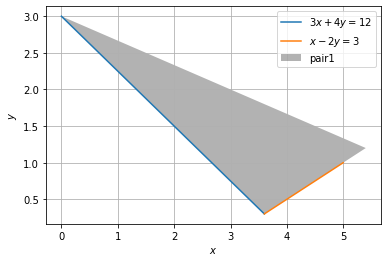
\includegraphics[width=\columnwidth]{solutions/su2021/2/56/Figure9_1.png}
    \caption{Inequality pair 1}
    \label{ineq/56/fig:inequalities1}	
    \end{figure}
    
    \begin{figure}[!ht]
    \centering
    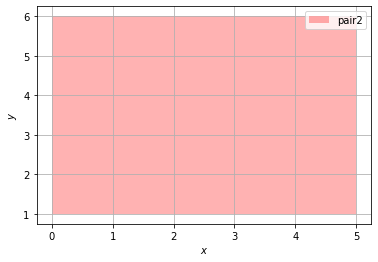
\includegraphics[width=\columnwidth]{solutions/su2021/2/56/Figure9_2.png}
    \caption{Inequality pair 2}
    \label{ineq/56/fig:inequalities2}	
    \end{figure}
    
    \begin{figure}[!ht]
    \centering
    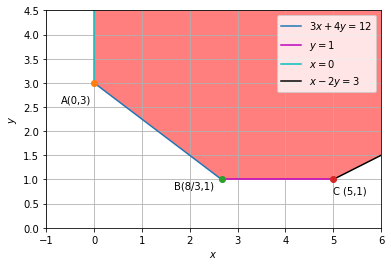
\includegraphics[width=\columnwidth]{solutions/su2021/2/56/Figure 9_3.png}
    \caption{Intersection of \ref{ineq/56/fig:inequalities1} and \ref{ineq/56/fig:inequalities2}}
    \label{ineq/56/fig:inequality3}	
    \end{figure}
    The common region shown by \ref{ineq/56/fig:inequality3} is the solution of set of inequalities.
    
\item Show that the points 
\begin{align}
\vec{A} = \myvec{2\\-1 \\1},
\vec{B} = \myvec{1\\-3 \\-5},
\vec{C} = \myvec{3\\ -4\\-4}
\end{align}
%
are the vertices of a right angled triangle.
\\
\solution

\begin{align}
\because \myvec{\vec{A-C}}^\top\myvec{\vec{B-C}}=\myvec{-1&3&5}\myvec{-2\\1\\-1}\\=0
\end{align}
the triangle in Fig.     \ref{fig:vec/2/4/} is right angled.
\begin{figure}[ht]
    \centering
    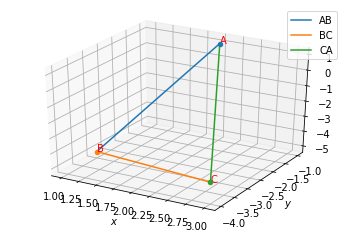
\includegraphics[width=\columnwidth]{solutions/su2021/2/4/Right angle triangle.png}
    \caption{}
    \label{fig:vec/2/4/}
    \end{figure} 




\item In $\triangle ABC$, 
$
\vec{A} = \myvec{1\\2 \\3},
\vec{B} = \myvec{-1\\0 \\0},
\vec{C} = \myvec{0\\ 1\\2}.
$
Find $\angle B$.
\\
\solution
We obtain the vertices of the rhombus as follows
\begin{align}
\vec{A} = \myvec{-3\\0},
\vec{B} = \myvec{0\\-3.5},
\vec{C} = \myvec{3\\0},
\vec{D} = \myvec{0\\3.5}
\end{align}
which are plotted in Fig. \ref{quad/45/fig:Rhombus ABCD}.
%
\begin{figure}[ht!]
\centering
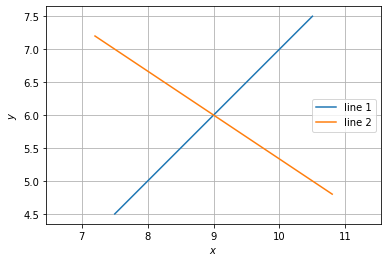
\includegraphics[width=\columnwidth]{solutions/quad/45/figure2.png}
\caption{Rhombus ABCD}
\label{quad/45/fig:Rhombus ABCD}
\end{figure}

\item Find the area of a triangle having the points 
$
\vec{A} = \myvec{1\\1 \\1},
\vec{B} = \myvec{1\\2 \\3}, \text{ and }
\vec{C} = \myvec{2\\ 3\\1}
$
as its vertices.
\\
\solution
From the given information, 
%
\begin{align}
    \vec{B-A}=\myvec{1\\2\\3}-\myvec{1\\1\\1} = \myvec{0\\1\\2}\\
    \vec{C-A}=\myvec{2\\3\\1}-\myvec{1\\1\\1}=\myvec{1\\2\\0}\\
    \end{align}
The area of a triangle using the vector product is then obtained as
\begin{align}
    \frac{1}{2}\norm{\myvec{\vec{B-A}}\times\myvec{\vec{C-A}}}\\ \frac{1}{2}\norm{\myvec{0\\1\\2}\times \myvec{1\\2\\0}}\\=1
    \end{align}
%
\item Find the area of a triangle with vertices
$
\vec{A} = \myvec{1\\1 \\2},
\vec{B} = \myvec{2\\3 \\5}, \text{ and }
\vec{C} = \myvec{1\\ 5\\5}
$
\\
\solution
From the given information, 
%
\begin{align}
\vec{B-A}&=\myvec{2\\3\\5}-\myvec{1\\1\\2} = \myvec{1\\2\\3}\\
\vec{C-A}&=\myvec{1\\5\\5}-\myvec{1\\1\\2}=\myvec{0\\4\\3}
\end{align}
The area of a triangle using the vector product is then obtained as
\begin{align}
        \frac{1}{2}\norm{\myvec{\vec{B-A}}\times\myvec{\vec{C-A}}} \\=\frac{1}{2}\norm{\myvec{1\\2\\3}\times \myvec{0\\4\\3}}\\=\frac{17}{2}
    \end{align}
\item Show that 
$
\vec{A}=\myvec{2\\3\\-4}, 
\vec{B}=\myvec{1\\-2\\3} \text{ and } 
\vec{C}=\myvec{3\\8\\-11}$  
are collinear.
\\
\solution 
%
We obtain the vertices of the rhombus as follows
\begin{align}
\vec{A} = \myvec{-3\\0},
\vec{B} = \myvec{0\\-3.5},
\vec{C} = \myvec{3\\0},
\vec{D} = \myvec{0\\3.5}
\end{align}
which are plotted in Fig. \ref{quad/45/fig:Rhombus ABCD}.
%
\begin{figure}[ht!]
\centering
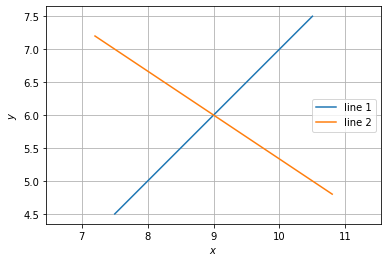
\includegraphics[width=\columnwidth]{solutions/quad/45/figure2.png}
\caption{Rhombus ABCD}
\label{quad/45/fig:Rhombus ABCD}
\end{figure}

\item Find the equation of set of points $\vec{P}$ such that
\begin{align}
PA^2+PB^2 =2k^2,
\end{align}
%
\begin{align}
\vec{A} = \myvec{3\\4 \\5},
\vec{B} = \myvec{-1\\3 \\-7},
\end{align}
%
respectively.
%
%
\solution
Let,
\begin{align}
 \vec P &=\vec{X};
\end{align}
 so,
 \begin{align}
 \vec{(PA)}^2&=\norm{\vec P-\vec A}^2\\
 &=\norm{\vec X-\vec A}^2\\
 &=\norm{\vec X}^2+\norm{\vec A}^2-2\vec X^T\vec A\label{vec/25/eq1}
 \end{align}
 and
 \begin{align}
 \vec{(PB)}^2&=\norm{\vec P-\vec B}^2\\
 &=\norm{\vec X-\vec B}^2\\
 &=\norm{\vec X}^2+\norm{\vec B}^2-2\vec X^T\vec B\label{vec/25/eq2}
 \end{align}
 The given equation is
\begin{align}
 \vec{(PA)}^2+ \vec{(PB)}^2 =2k^2\label{vec/25/eq3}
 \end{align}
 Sub \eqref{vec/25/eq1} and \eqref{vec/25/eq2}   values in \eqref{vec/25/eq3} 
\begin{align}
\norm{\vec X}^2+\norm{\vec A}^2-2\vec X^T\vec A+\norm{\vec X}^2+\norm{\vec B}^2-2\vec X^T\vec B=2k^2\\
\implies 2\norm{\vec X}^2+\norm{\vec A}^2+\norm{\vec B}^2-2\vec X^T(\vec A+\vec B)=2k^2\label{vec/25/eq4} 
\end{align}
sub $\vec A$,$\vec B$ values in equation \eqref{vec/25/eq4} ,we get
\begin{align}
 2\norm{\vec X}^2+\norm{\myvec{3\\4\\5}}^2+\norm{\myvec{-1\\3\\-7}}^2-2\vec X^T\brak{\myvec{3\\4\\5}+\myvec{-1\\3\\-7}}=2k^2
 \end{align}
 $\therefore$ the required equation is
 \begin{align}
  2\norm{\vec X}^2-2\vec X^T\myvec{2\\7\\-2}+109-2k^2=0
\end{align}   

\item Find the coordinates of a point which divides the line segment joining the points \myvec{1\\-2\\3} and \myvec{3\\4\\-5} in the ratio $2:3$
\begin{enumerate}
\item internally, and
\item externally.
\end{enumerate}
%
\solution
We obtain the vertices of the rhombus as follows
\begin{align}
\vec{A} = \myvec{-3\\0},
\vec{B} = \myvec{0\\-3.5},
\vec{C} = \myvec{3\\0},
\vec{D} = \myvec{0\\3.5}
\end{align}
which are plotted in Fig. \ref{quad/45/fig:Rhombus ABCD}.
%
\begin{figure}[ht!]
\centering
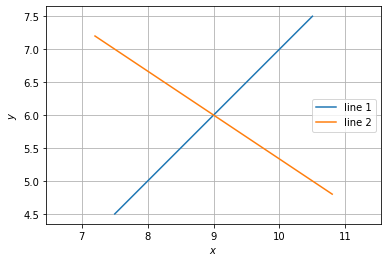
\includegraphics[width=\columnwidth]{solutions/quad/45/figure2.png}
\caption{Rhombus ABCD}
\label{quad/45/fig:Rhombus ABCD}
\end{figure}

%\solution Use \eqref{eq:line_section_form}.

\item Prove that the three points \myvec{-4\\6\\10}, \myvec{2\\4\\6} and \myvec{14\\0\\-2} are collinear.
%
\\
\solution 
%
We obtain the vertices of the rhombus as follows
\begin{align}
\vec{A} = \myvec{-3\\0},
\vec{B} = \myvec{0\\-3.5},
\vec{C} = \myvec{3\\0},
\vec{D} = \myvec{0\\3.5}
\end{align}
which are plotted in Fig. \ref{quad/45/fig:Rhombus ABCD}.
%
\begin{figure}[ht!]
\centering
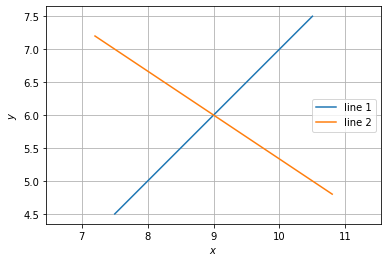
\includegraphics[width=\columnwidth]{solutions/quad/45/figure2.png}
\caption{Rhombus ABCD}
\label{quad/45/fig:Rhombus ABCD}
\end{figure}

\item Find the equation of the set of points $\vec{P}$ such that its distances from the points
$
\vec{A}=\myvec{3\\4\\-5}, 
\vec{B}=\myvec{-2\\1\\4}
$
are equal. 
\\
\solution
We obtain the vertices of the rhombus as follows
\begin{align}
\vec{A} = \myvec{-3\\0},
\vec{B} = \myvec{0\\-3.5},
\vec{C} = \myvec{3\\0},
\vec{D} = \myvec{0\\3.5}
\end{align}
which are plotted in Fig. \ref{quad/45/fig:Rhombus ABCD}.
%
\begin{figure}[ht!]
\centering
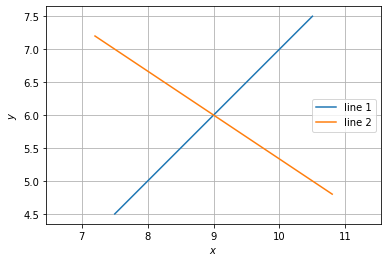
\includegraphics[width=\columnwidth]{solutions/quad/45/figure2.png}
\caption{Rhombus ABCD}
\label{quad/45/fig:Rhombus ABCD}
\end{figure}

\item The line through the points \myvec{-2\\6} and \myvec{4\\8} is perpendicular to the line through the points \myvec{8\\12} and $\myvec{x\\24}$.  Find the value of $x$.
\\
\solution
We obtain the vertices of the rhombus as follows
\begin{align}
\vec{A} = \myvec{-3\\0},
\vec{B} = \myvec{0\\-3.5},
\vec{C} = \myvec{3\\0},
\vec{D} = \myvec{0\\3.5}
\end{align}
which are plotted in Fig. \ref{quad/45/fig:Rhombus ABCD}.
%
\begin{figure}[ht!]
\centering
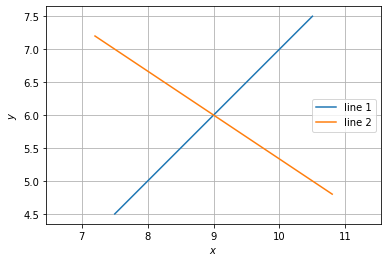
\includegraphics[width=\columnwidth]{solutions/quad/45/figure2.png}
\caption{Rhombus ABCD}
\label{quad/45/fig:Rhombus ABCD}
\end{figure}

\item Show that the line joining the origin to the point \myvec{2\\1\\1} is perpendicular to the line determined by the points \myvec{3\\5\\-1}, \myvec{4\\3\\-1}.
\\
\solution
Let 
\begin{align}
 \vec{O}=\myvec{0\\0\\0}, 
 \vec{P}=\myvec{2\\1\\1} ,\vec{A}=\myvec{3\\5\\-1} ,\vec{B}=\myvec{4\\3\\-1}  
\end{align}
Then,
\begin{align}
\vec{O}-\vec{P}&=\myvec{2\\1\\1}
\\
&=\myvec{4\\3\\-1}-\myvec{3\\5\\-1}
\\
\vec{A}-\vec{B}&=\myvec{1\\-2\\0}
\end{align}
and 
\begin{align}
\brak{\vec{O}-\vec{P}}^T(\vec{A}-\vec{B})=0
\\
\implies \brak{\vec{O}-\vec{P}} \perp \brak{\vec{A}-\vec{B}}
\end{align}

%
%
%\end{enumerate}
%
 
\input{./quad/quad_geo_exam.tex} 
\input{./line/coord_ex.tex}
\input{./line/section.tex}
\input{./line/complex.tex}
\input{./line/line_motion.tex}

\end{enumerate}

\section{Exercises}
\renewcommand{\theequation}{\theenumi}
\begin{enumerate}[label=\thesection.\arabic*.,ref=\thesection.\theenumi]
\numberwithin{equation}{enumi}
%\renewcommand{\theequation}{\theenumi}
%\begin{enumerate}[label=\arabic*.,ref=\thesubsection.\theenumi]
%\numberwithin{equation}{enumi}
%
\item The vertices of $\triangle ABC$ are $\vec{A}=\myvec{4\\6},  \vec{B}=\myvec{1\\5}$ and  $\vec{C} =  \myvec{7\\2}$.  A line is drawn to intersect sides $AB$ and $AC$ at $D$ and $E$ respectively, such that
\begin{align}
\frac{AD}{AB}=\frac{AE}{AC}= \frac{1}{4}
\end{align}
%
Find 
\begin{align}
\frac{\text{area of }\triangle ADE}{\text{area of }\triangle ABC}.
\end{align}
\item Let $\vec{A}=\myvec{4\\2},  \vec{B}=\myvec{6\\5}$ and  $\vec{C} =  \myvec{1\\4}$ be the vertices of $\triangle ABC$.
\begin{enumerate}
\item The median from $\vec{A}$ meets $BC$ at $\vec{D}$.  Find the coordinates of the point $\vec{D}$.
\item Find the coordinates of the point $\vec{P}$ on $AD$ such that $AP:PD = 2:1$.
\item Find the coordinates of the points $\vec{Q}$ and $\vec{R}$ on medians $BE$ and $CF$ respectively such that $BQ:QE = 2:1$ and $CR:RF = 2:1$.
\end{enumerate}
\solution



\begin{figure}[!ht]
    \centering
    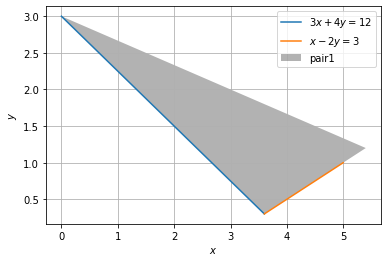
\includegraphics[width=\columnwidth]{solutions/su2021/2/56/Figure9_1.png}
    \caption{Inequality pair 1}
    \label{ineq/56/fig:inequalities1}	
    \end{figure}
    
    \begin{figure}[!ht]
    \centering
    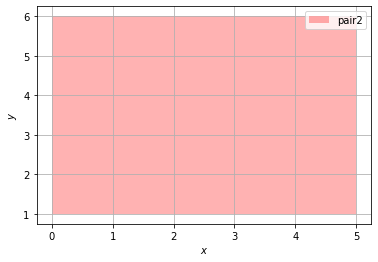
\includegraphics[width=\columnwidth]{solutions/su2021/2/56/Figure9_2.png}
    \caption{Inequality pair 2}
    \label{ineq/56/fig:inequalities2}	
    \end{figure}
    
    \begin{figure}[!ht]
    \centering
    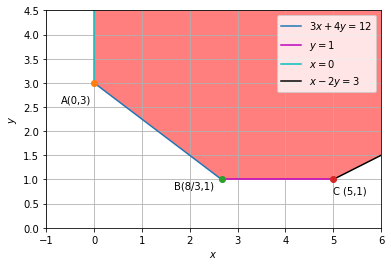
\includegraphics[width=\columnwidth]{solutions/su2021/2/56/Figure 9_3.png}
    \caption{Intersection of \ref{ineq/56/fig:inequalities1} and \ref{ineq/56/fig:inequalities2}}
    \label{ineq/56/fig:inequality3}	
    \end{figure}
    The common region shown by \ref{ineq/56/fig:inequality3} is the solution of set of inequalities.
    
\item In $\triangle ABC$, Show that the centroid 
\begin{align}
\vec{O} = \frac{\vec{A}+\vec{B}+\vec{C}}{3}
\end{align}
\item Show that the points 
\begin{align}
\vec{A} = \myvec{2\\-1 \\1},
\vec{B} = \myvec{1\\-3 \\-5},
\vec{C} = \myvec{3\\ -4\\-4}
\end{align}
%
are the vertices of a right angled triangle.
\item In $\triangle ABC$, 
$
\vec{A} = \myvec{1\\2 \\3},
\vec{B} = \myvec{-1\\0 \\0},
\vec{C} = \myvec{0\\ 1\\2}.
$
Find $\angle B$.
\\
\solution
We obtain the vertices of the rhombus as follows
\begin{align}
\vec{A} = \myvec{-3\\0},
\vec{B} = \myvec{0\\-3.5},
\vec{C} = \myvec{3\\0},
\vec{D} = \myvec{0\\3.5}
\end{align}
which are plotted in Fig. \ref{quad/45/fig:Rhombus ABCD}.
%
\begin{figure}[ht!]
\centering
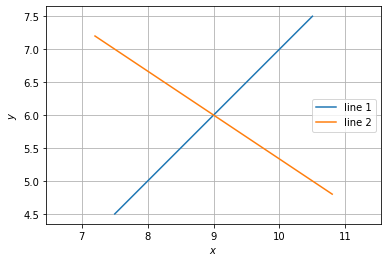
\includegraphics[width=\columnwidth]{solutions/quad/45/figure2.png}
\caption{Rhombus ABCD}
\label{quad/45/fig:Rhombus ABCD}
\end{figure}


\item Show that the vectors 
$
\myvec{2\\-1 \\1},
\myvec{1\\-3 \\-5},
\myvec{3\\ -4\\-4}
$
form the vertices of a right angled triangle.
\item Find the area of a triangle having the points 
$
\vec{A} = \myvec{1\\1 \\1},
\vec{B} = \myvec{1\\2 \\3}, \text{ and }
\vec{C} = \myvec{2\\ 3\\1}
$
as its vertices.
\item Find the area of a triangle with vertices
$
\vec{A} = \myvec{1\\1 \\2},
\vec{B} = \myvec{2\\3 \\5}, \text{ and }
\vec{C} = \myvec{1\\ 5\\5}
$
\item Find the direction vectors of the sides of a triangle with vertices
$
\vec{A} = \myvec{3\\5 \\-4},
\vec{B} = \myvec{-1\\1 \\2}, \text{ and }
\vec{C} = \myvec{-5\\ -5\\-2}
$
\item Check whether 
\begin{align}
\myvec{5\\-2}, \myvec{6\\4}, \myvec{7\\-2}
\end{align}
are the vertices of an isosceles triangle.
%
 \item Are the points 
\begin{align}
\vec{A} = \myvec{3\\6 \\9},
\vec{B} = \myvec{10\\20 \\30},
\vec{C} = \myvec{25\\ -41\\5},
\end{align}
%
the vertices of a right angled triangle?
\item Determine if the points 
\begin{align}
\myvec{1\\5}, \myvec{2\\3}, \myvec{-2\\-11}
\end{align}
%
are collinear.	
\item By using the concept of equation of a line, prove that the three points \myvec{3\\ 0}, \myvec{– 2\\ – 2} and \myvec{8\\ 2} are collinear.
\item Find the value of $x$ for which the points $\myvec{x\\ – 1}$, \myvec{2\\1} and \myvec{4\\ 5} are collinear.
\item  In each of the following, find the value of $k$ for which the points are collinear

\begin{enumerate}
\item \myvec{7\\-2},  \myvec{5\\1},  \myvec{3\\k} 
\item \myvec{8\\1},  \myvec{k\\-4},  \myvec{2\\-5} 
\end{enumerate}
\item Find a condition on $\vec{x}$  such that the points $\vec{x}, \myvec{1\\2}\myvec{7\\0}$ are collinear.
\item Show that the points 
$\vec{A}=\myvec{1\\2\\7}, \vec{B}=\myvec{2\\6\\3}$ and $ \vec{C}=\myvec{3\\10\\-1}$ are collinear.
\item Show that the points 
$\vec{A}=\myvec{1\\-2\\8}, \vec{B}=\myvec{5\\0\\-2}$ and $ \vec{C}=\myvec{11\\3\\7}$ are collinear, and find the ratio in which $\vec{B}$ divides $AC$.
\item Show that 
$
\vec{A}=\myvec{2\\3\\4}, 
\vec{B}=\myvec{-1\\-2\\1} \text{ and } 
\vec{C}=\myvec{5\\8\\7}$  
are collinear.

\item A bullet fired at an angle of 30$\degree$ with the horizontal hits the ground 3.0 km away. By adjusting its angle of projection, can one hope to hit a target 5.0 km away ? Assume the muzzle speed to be fixed, and neglect air resistance.
\item  A fighter plane flying horizontally at an altitude of 1.5 km with speed 720 km/h passes directly overhead an anti-aircraft gun. At what angle from the vertical should the gun be fired for the shell with muzzle speed 600 $m s^{-1}$ to hit the plane ? 
At what minimum  altitude should the pilot fly the plane to avoid being hit ? (Take g = 10$ m s^{-2}$
).
\item Give the magnitude and direction of the net force acting on a stone of mass 0.1 kg, 
\begin{enumerate}
\item  just after it is dropped from the window of a stationary train, 
\item  just after it is dropped from the window of a train running at a constant velocity of 36 km/h,
\item  just after it is dropped from the window of a train accelerating with 1$ m s^{-2} $
\item  lying on the floor of a train which is accelerating with 1 $m s^{-2}$, the stone being at rest relative to the train.
\end{enumerate}
Neglect air resistance throughout. 

\item Consider the collision depicted in Fig. \ref{fig:6.10} to be between two billiard balls with equal masses $m_1= m_2$.  The first ball is called the cue while the second ball is called the target. The billiard player wants to 'sink' the target ball in a corner pocket, which is at an angle $\theta_2=37\degree$.  Assume that the collosion
is elastic and that friction and rotational motion are not important. Obtain $\theta_1$.
\begin{figure}[!ht]
\centering
\includegraphics[width=\columnwidth]{./line/figs/11-1/6/6.10.eps}
\caption{}
\label{fig:6.10}
\end{figure}
\item Show that 
$
\vec{A}=\myvec{2\\3\\-4}, 
\vec{B}=\myvec{1\\-2\\3} \text{ and } 
\vec{C}=\myvec{3\\8\\-11}$  
are collinear.
\\
\solution 
%
We obtain the vertices of the rhombus as follows
\begin{align}
\vec{A} = \myvec{-3\\0},
\vec{B} = \myvec{0\\-3.5},
\vec{C} = \myvec{3\\0},
\vec{D} = \myvec{0\\3.5}
\end{align}
which are plotted in Fig. \ref{quad/45/fig:Rhombus ABCD}.
%
\begin{figure}[ht!]
\centering
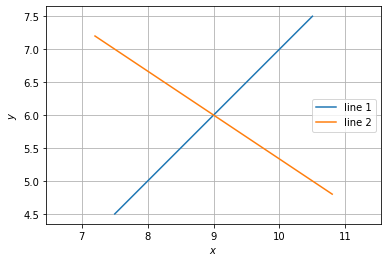
\includegraphics[width=\columnwidth]{solutions/quad/45/figure2.png}
\caption{Rhombus ABCD}
\label{quad/45/fig:Rhombus ABCD}
\end{figure}

\item Find the equation of set of points $\vec{P}$ such that
\begin{align}
PA^2+PB^2 =2k^2,
\end{align}
%
\begin{align}
\vec{A} = \myvec{3\\4 \\5},
\vec{B} = \myvec{-1\\3 \\-7},
\end{align}
%
respectively.
%
\item Find the coordinates of a point which divides the line segment joining the points \myvec{1\\-2\\3} and \myvec{3\\4\\-5} in the ratio $2:3$
\begin{enumerate}
\item internally, and
\item externally.
\end{enumerate}
%
\solution
We obtain the vertices of the rhombus as follows
\begin{align}
\vec{A} = \myvec{-3\\0},
\vec{B} = \myvec{0\\-3.5},
\vec{C} = \myvec{3\\0},
\vec{D} = \myvec{0\\3.5}
\end{align}
which are plotted in Fig. \ref{quad/45/fig:Rhombus ABCD}.
%
\begin{figure}[ht!]
\centering
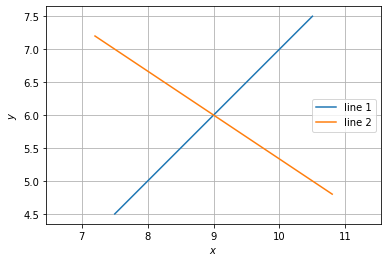
\includegraphics[width=\columnwidth]{solutions/quad/45/figure2.png}
\caption{Rhombus ABCD}
\label{quad/45/fig:Rhombus ABCD}
\end{figure}

%\solution Use \eqref{eq:line_section_form}.

\item Prove that the three points \myvec{-4\\6\\10}, \myvec{2\\4\\6} and \myvec{14\\0\\-2} are collinear.
%
\\
\solution 
%
We obtain the vertices of the rhombus as follows
\begin{align}
\vec{A} = \myvec{-3\\0},
\vec{B} = \myvec{0\\-3.5},
\vec{C} = \myvec{3\\0},
\vec{D} = \myvec{0\\3.5}
\end{align}
which are plotted in Fig. \ref{quad/45/fig:Rhombus ABCD}.
%
\begin{figure}[ht!]
\centering
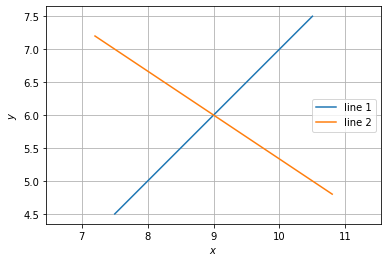
\includegraphics[width=\columnwidth]{solutions/quad/45/figure2.png}
\caption{Rhombus ABCD}
\label{quad/45/fig:Rhombus ABCD}
\end{figure}

%
\item Find the ratio in which the line segment joining the points \myvec{4\\8\\10} and \myvec{6\\10\\-8} is divided by the YZ-plane.
%
%\\
%\solution Use \eqref{eq:line_section_form}.  The YZ-plane has points \myvec{0\\y\\z}.
%
\item Find the equation of the set of points $\vec{P}$ such that its distances from the points
$
\vec{A}=\myvec{3\\4\\-5}, 
\vec{B}=\myvec{-2\\1\\4}
$
are equal. 
%
%\\
%\solution Use the approach in Problem \ref{prob:line_perp_bisect}.
\item If 
\begin{align}
\vec{P} = 3\vec{a}-2\vec{b}
\\
\vec{Q} = \vec{a}+\vec{b}
\end{align}
%
find $\vec{R}$, which divides $PQ$ in the ratio $2:1$
\begin{enumerate}
\item internally,
\item externally.
\end{enumerate}
%
\item Find a unit vector in the direction of \myvec{2\\-1\\-2}.
%
\item Find a unit vector in the direction of the line passing through \myvec{-2\\4\\-5} and $\myvec{1\\2\\3}$.
%
\item Find a unit vector in the direction of $\vec{a}+\vec{b}$, where 
%
\begin{align}
\vec{a} = \myvec{2\\2\\-5}, \vec{b} = \myvec{2\\1\\3}.
\end{align}
%
\item Find a unit vector in the direction of 
%
\begin{align}
\myvec{1\\1\\-2}.
\end{align}
%
\item Find a point on the $y$-axis which is equidistant from the points $\vec{A} = \myvec{6\\5}, \vec{B} = \myvec{-4\\3}$.

\item The line through the points \myvec{-2\\6} and \myvec{4\\8} is perpendicular to the line through the points \myvec{8\\12} and $\myvec{x\\24}$.  Find the value of $x$.

%\end{enumerate}
%

 
\input{./quad/quad_geo.tex} 
\end{enumerate}
%%
%%
\end{document}


